\documentclass{beamer} % Use handout to get rid of repeated slides
\usetheme{AnnArbor}
\usecolortheme{default}
\usefonttheme{professionalfonts}
\usepackage{mathpazo}
\usepackage{listings}
\usepackage{xcolor}

% Define colors
\definecolor{myred}{RGB}{163,0,0}
\definecolor{ttcolor}{RGB}{0,0,1}%{RGB}{163,0,0}
\definecolor{mygray}{RGB}{248,249,250} 
\definecolor{mygreen1}{RGB}{0,96,0}
\definecolor{mygreen2}{RGB}{229,239,229}
\definecolor{aristotelgreen}{HTML}{008A44}
\definecolor{aristotelred}{HTML}{9E0101}
\definecolor{aristotelgrey}{HTML}{2E2E2E}
\definecolor{aristoteldarkred}{HTML}{500101}
\definecolor{aristotelorange}{HTML}{FF8C00}

\setbeamertemplate{theorem}[ams style]
\setbeamertemplate{theorems}[numbered]

\usepackage{etoolbox}

\undef{\definition}
\theoremstyle{definition}
\newtheorem{definition}{\translate{Definition}}
\hypersetup{
	colorlinks=true,
	linkcolor=aristotelorange,   % color for normal internal links
	citecolor=aristotelgreen,   % color for citation links
	urlcolor=aristotelgreen      % color for external links
}

\setbeamercolor{palette primary}{bg=aristotelred, fg=white}
\setbeamercolor{palette secondary}{bg=aristoteldarkred, fg=white}
\setbeamercolor{palette tertiary}{bg=black, fg=white} 

\setbeamercolor{title}{fg=white, bg=aristotelred} % Title text color
\setbeamercolor{subtitle}{fg=white, bg=aristotelred} % Subtitle text color
\setbeamercolor{background canvas}{bg=aristotelgrey} % Background for content canvas
\setbeamercolor{normal text}{fg=white} % Normal text color
\setbeamercolor{titlegraphic}{bg=mygray} % Background color for title graphic area
\setbeamercolor{frametitle}{fg=white, bg=aristoteldarkred}

% Change color of numbered circles in the table of contents
\setbeamercolor{section number projected}{bg=white, fg=black}
\setbeamercolor{subsection number projected}{bg=aristotelred, fg=aristotelgrey}
\setbeamercolor{subsection number projected}{bg=aristotelorange, fg=white}

\setbeamercolor{block title}{fg=white,bg=mygreen1}
\setbeamercolor{block body}{fg=black,bg=mygreen2}


\lstdefinestyle{rstyle}%
{language=[LaTeX]TeX,
	basicstyle=\footnotesize\ttfamily,
	backgroundcolor = \color{mygray},
	commentstyle=\slshape\color{green!50!black},
	keywordstyle=\color{blue},
	identifierstyle=\color{blue},
	stringstyle=\color{orange},
	%escapechar=\#,
	rulecolor = \color{mygray}, 
	showstringspaces = false,
	showtabs = false,
	tabsize = 2,
	emphstyle=\color{red},
	frame = single} 

\begin{document}
	\title[Paper presentation]{Presentation of a paper:}
	\subtitle[subtitle?]{The Economic Costs of Conflict: 
		A Case Study of the Basque Country \\
		A. Abadie \& J. Gardeazabal (2001) }
	\author[Riste Petrov]{Riste Petrov \\ \href{mailto:riste@uni-sofia.bg}{riste@uni-sofia.bg}}
	\institute[AEEM - FEBA]{AEEM - FEBA - Sofia University St. Kliment Ohridski - coh. 2026/27}
	\titlegraphic{\includegraphics[scale=0.5]{/home/anonymous/Documents/Mega/ЦЕЛ/Master/1Courses/SU ENG White horizontal.pdf}}
	\date{\today}
	
	\begin{frame}[fragile]
		\titlepage
	\end{frame}
	
	\begin{frame}[fragile]
		\frametitle{Contents}
		\tableofcontents[]
	\end{frame}

	\section{Introduction}
	\subsection{Authors}
	\begin{frame}[fragile]
		\frametitle{Background of the authors}
		\framesubtitle{Academic}
		\textbf{Alberto Abadie}\\
		currently a professor of Economics at MIT, at the time of writing assistant professor at Harvard.\\

		\vspace{1em}
		\textbf{Javier Gardeazabal}\\
		currently a professor at the University of the Basque Country, Phd at the University of Pennsylvania in May 1991.
	\end{frame}
	
	\subsection{Some context}
	\begin{frame}[fragile]
		\frametitle{Basque during Franco and post Franco}
		\textbf{Franco Basque}\\
		Under Franco, the Basque Country suffered political repression and centralized economic policies that constrained regional autonomy and industrial investment, reducing long-term growth potential. Despite this the Basque region in the 1960s got one of the highest GDP per Capita, investment ration (investment/production), density of population, educated labor force in the whole of Spain.
		\\
		
		\vspace{1em}
		\textbf{post Franco Basque:}\\
		After Franco, democratization and restored regional authority allowed economic recovery and stronger institutions, but violence from ETA continued to impose measurable economic losses.
	\end{frame}
	
	\begin{frame}[fragile]
		 \frametitle{Basque during Franco and post Franco} 
		  \begin{minipage}[t]{0.48\textwidth} 
		  	\centering \textbf{Franco Basque}\\[0.5em] 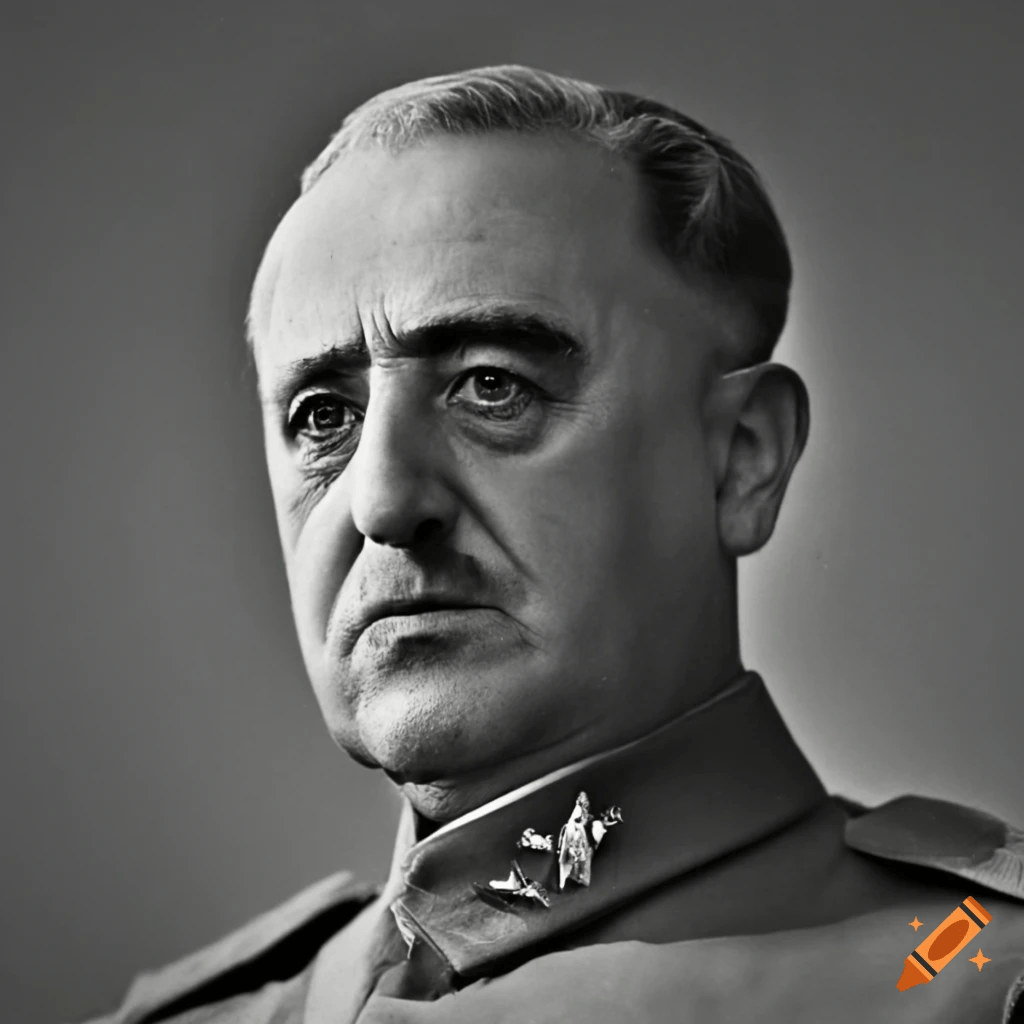
\includegraphics[width=\linewidth]{franco.png} 
		  \end{minipage}\hfill 
		  \begin{minipage}[t]{0.48\textwidth} 
		  	\centering \textbf{Post‑Franco Basque}\\[0.5em] 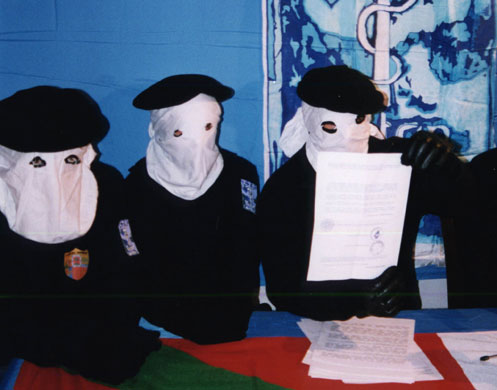
\includegraphics[width=\linewidth]{eta.jpg} 
	  	\end{minipage} 
  	\end{frame}
	
	\section{Research}
	\subsection{Scenario Model of GDP}
	\begin{frame}[fragile]
		\frametitle{How the Authors simulated the Counterfactual scenario?} 
		\begin{itemize}
			\item They compared the Basque Country’s observed economic path to a weighted combination of the 16 other Spanish regions to construct a “synthetic” Basque Country without terrorism.
			\item Choose nonnegative weights W that sum to one so the weighted average of control regions best matches Basque pre‑terrorism characteristics. Where V is adiagonal matrix weighting predictor of importance chosen empirically.
			\begin{equation*}
				(X_1 - X_0W)'V(X_1 - X_0W)
			\end{equation*}
			\item The resulting W* uses Catalonia (0.8508) and Madrid (0.1492) as positive-weight controls; others get zero weight. Assuming that Basque with keep up with the growth (Catalonia and Madrid retained) it had during Franco.
		\end{itemize}
	\end{frame}
	
	\begin{frame}[fragile]
		\frametitle{Synthetic \& Placebo} 
		\begin{minipage}[t]{0.48\textwidth} 
			\centering \textbf{Synthetic}\\[0.5em] 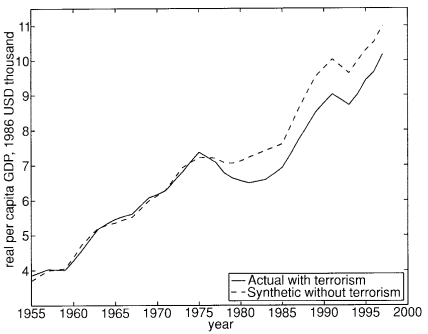
\includegraphics[width=\linewidth]{basque-syntethic.png} 
		\end{minipage}\hfill 
		\begin{minipage}[t]{0.48\textwidth} 
			\centering \textbf{Catalonia Placebo}\\[0.5em] 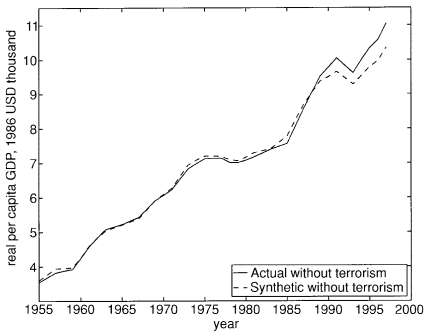
\includegraphics[width=\linewidth]{Catalonia.png} 
		\end{minipage} 
	\end{frame}
	
	\subsection{Stocks Modeling}
	\begin{frame}[fragile]
		\frametitle{Fama-French Models} 
		At the time of writing the 3 variable one was existent. The five model one was updated in 2015. 
		$$	r = R_f + \beta(R_m - R_f) + b_s \cdot SMB + b_v \cdot HML + b_p \cdot RMW_5 + b_i \cdot CMA_5 + \alpha   $$
		\begin{center}
			$R_f$ - Risk free return rate\\
			$R_m$ - Return of the market portfolio\\
			$SMB$ - Small market cap. - Big market cap. (returns)\\
			$HML$ - High B/M - Low B/M (returns)\\
			$RMW_5$ - High Operating prof. - Low Operating prof. (returns)\\
			$CMA_5$ - Conservative investing - Intensive investing (returns)\\ 
		\end{center}
		\vspace{1em}
		\begin{small}
			In the US (1963–2013), adding these two factors makes HML redundant: its returns are explained by the other four factors, especially CMA (corr $\approx$ 0.7).
		\end{small}
	\end{frame}
	
	\begin{frame}[fragile]
		\frametitle{Natural Experiment using the Truce of 1998-1999}
		The authors used in total 3 types of model to test out the causality of the effects of EPAs activity during the temporary truce.\\
		French-Fama 
		$$ R_t^j  = \alpha^j + \beta_1^jR_i^m + \beta_2^j SMB_t + \beta^j_3 HML_t + AR_t^j$$
		Noise-less day after the truce portfolio
		$$ CAR_t^j = \left( \prod_{s=1}^{t} \left\{1+AR_s^j\right\} \right) - 1 $$
		Market Model
		$$ R_t^j  = \gamma^j + \lambda R_t^m + AR_t^j $$
		Constant Mean Return
		$$ R_t^j  = \mu^j + AR_t^j $$
		
	\end{frame}
	
	\begin{frame}[fragile]
		\frametitle{Noise-less day after truce portfolio comparison}
		\begin{center}
			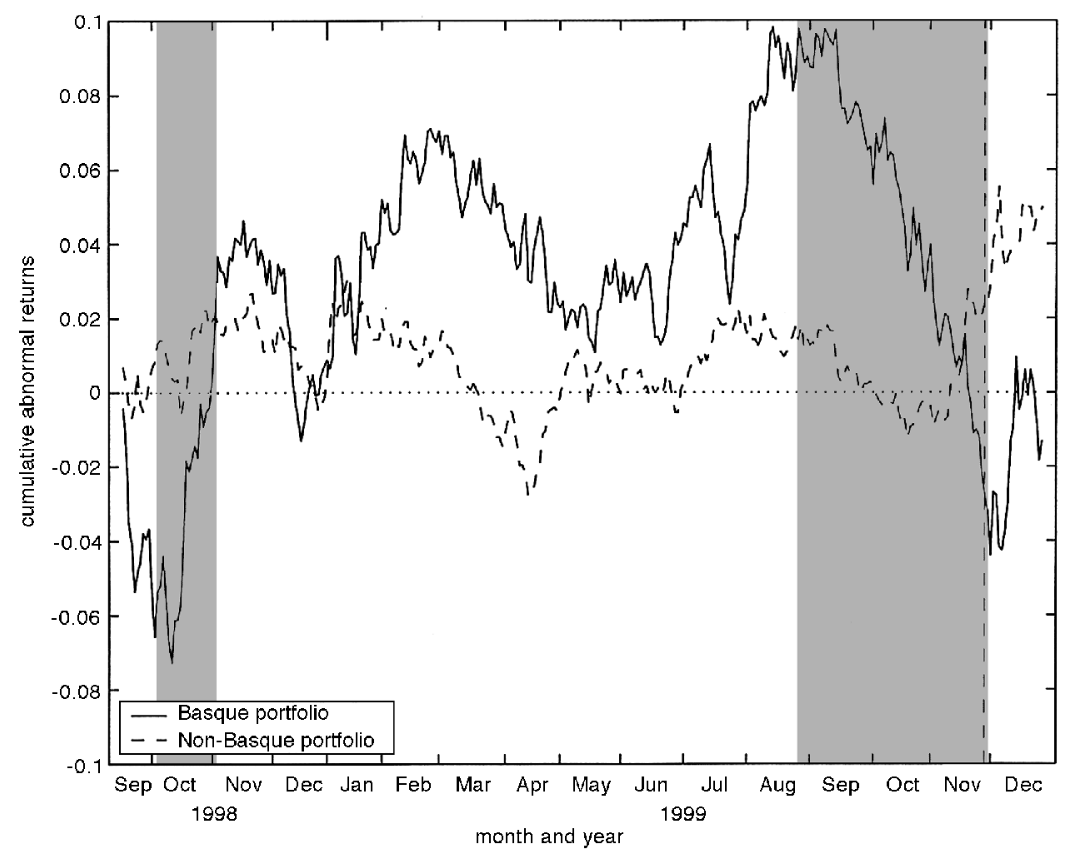
\includegraphics[width=0.8\textwidth,height=0.8\textheight]{truce.png} 
		\end{center}
	\end{frame}
	
	\begin{frame}[fragile]
		\frametitle{Comparison of coefficients of the three main models}
		\begin{center}
			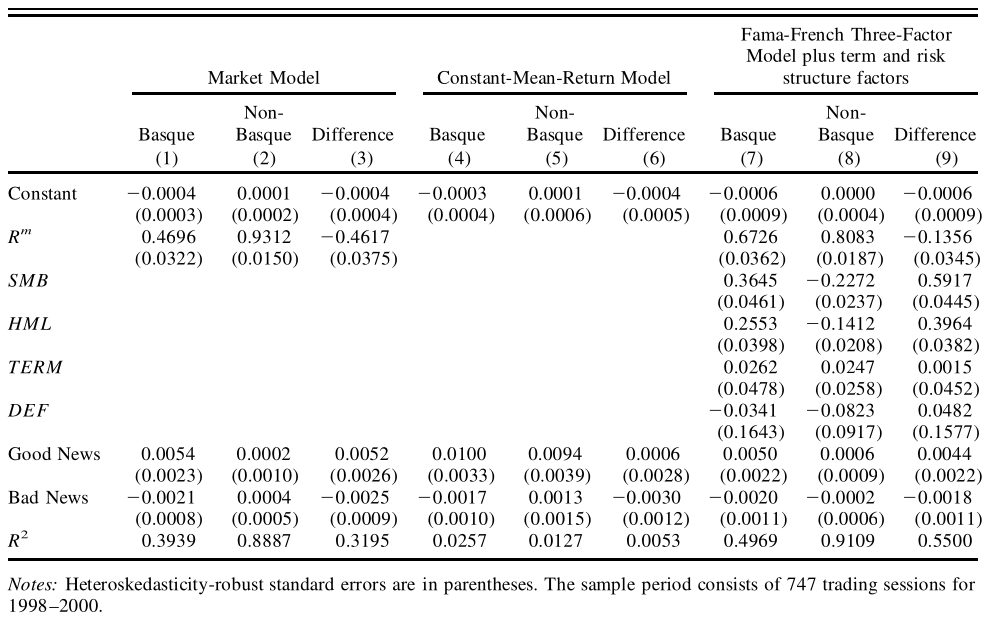
\includegraphics[width=0.8\textwidth,height=0.8\textheight]{models.png} 
		\end{center}
	\end{frame}
	
	
	\section{Q\&A}
	\begin{frame}[fragile]
		\frametitle{Ending remarks}
		\begin{center}
			I am delighted for your attention.\\
			\vspace{1em}
			Q \& A?
		\end{center}
	\end{frame}
	
\end{document}